\section{Resoconto delle attività di verifica}

In questa sezione vengono inserite tutte le misurazioni delle metriche trovate dal gruppo \gruppo.
Il team si impegna a garantire almeno il soddisfacimento del range di accettazione per ogni metrica.

Per quanto riguarda le misurazioni può essere calcolato un risultato singolo, se la metrica si riferisce ad una caratteristica singola, oppure può essere calcolato un risultato massimo, ovvero una metrica che si riferisce a più componenti, ad esempio le classi. In tal caso verrà presa la misurazione peggiore e confrontata con i valori scelti dal team precedentemente.

Alcune metriche, infine, sono state misurate più volte nel tempo e per queste verrà illustrato un diagramma cartesiano, in cui: l'asse delle ascisse rappresenterà in giorni la durata del periodo fino alla consegna, mentre l'asse delle ordinate rappresenterà i valori assunti al momento delle misurazioni. \\
Verranno comunque riportati i risultati finali di tali metriche nell'apposita tabella.


\subsection{Revisione dei Requisiti}
In questa sezione vengono inseriti i risultati relativi al periodo di Revisione dei Requisiti e le metriche relative ad esso.

\subsubsection{Analisi statica dei documenti}
L'analisi statica dei documenti è stata fatta mediante \termine{Walkthrough} ed ha portato all'individuazione di alcuni errori. Tra gli errori individuati quelli più frequenti sono stati:
		\begin{itemize}
			\item Errori nei concetti esposti.
			\item Aggettivi o verbi utilizzati in modo scorretto.
			\item Periodi troppo lunghi o complessi da capire ed interpretare.
		\end{itemize}

\subsubsection{Esiti verifiche automatizzate}
		
\paragraph{Indice di Gulpease}

\begin{table}[h]
	\begin{center}
		\begin{tabular}{|c|c|c|c|}
			\hline
			\textbf{Documento}	& \textbf{Risultato} & \textbf{Esito} & \textbf{Valore} \\
			\hline
		 \termine{Analisi} dei Requisiti v1.0.0 & 90 & Superato & Ottimale	\\
			\hline
			Glossario v1.0.0 & 56 & Superato & Ottimale	\\
			\hline
			Norme di Progetto v1.0.0 & 47 & Superato & Accettabile \\
			\hline
			Piano di Progetto v1.0.0 & 48 & Superato & Accettabile\\
			\hline
			Piano di Qualifica v1.0.0	& 48 & Superato & Accettabile\\
			\hline
			Studio di Fattibilità v1.0.0	& 47 & Superato & Accettabile\\
			\hline
			Verbale\_Esterno\_1\_20161223 v1.0.0	& 51 & Superato & Ottimale	\\
			\hline
		\end{tabular}
	\end{center}
	\caption{RR - Risultato indice di Gulpease}
\end{table}

\subsubsection{Soddisfacimento metriche}

\paragraph{Qualità di processo}
\begin{longtable}{|>{\centering}m{5cm}|c|c|c|c|c|}
\hline
\textbf{Metrica} & \textbf{Unità di misura} & \textbf{Risultato} & \textbf{Risultato Massimo} & \textbf{Esito} & \textbf{Valore}\\
\hline
\endhead

\emph{Schedule Variance} & {Attività} & \textcolor{Green}{0} & / & Superato & Ottimale\\ \hline
\emph{Budget Variance} & {Euro} & \textcolor{Green}{15} & / & Superato & Ottimale \\ \hline
\emph{Rischi non preventivati} & {Rischi} & \textcolor{Green}{0} & / & Superato & Ottimale\\ \hline
\emph{Ottimalità delle misurazioni} & {Percentuale} & \textcolor{Green}{0.6} & / & Superato & Ottimale \\ \hline
\emph{Rischi non preventivati} & {Rischi} & \textcolor{Green}{0} & / & Superato & Ottimale\\ \hline
%\emph{Efficienza di gestione dei rischi} & {Giorni} & \textcolor{Orange}{21.3} & $\geq 20$ & $\geq 60$\\ \hline
%\emph{Requisiti obbligatori soddisfatti} & {Percentuale} & \textcolor{Green}{100} & $100$ & $100$\\ \hline
%\emph{Livello di stabilità-SDK} & {Percentuale} & / &\textcolor{Green}{1} & Accettabile\\ \hline
%\emph{Livello di stabilità-Applicazione} & {Percentuale} & / &\textcolor{Green}{1} & Accettabile\\ \hline
%\emph{Astrattezza-SDK} & {Percentuale} & / &\textcolor{Green}{0.8} & Accettabile\\ \hline
%\emph{Astrattezza-Applicazione} & {Percentuale} & / &\textcolor{Green}{0.5} & Ottimale\\ \hline
%\emph{Distanza dalla sequenza principale-SDK} & {Percentuale} & / &\textcolor{Green}{1} & Accettabile\\ \hline
%\emph{Distanza dalla sequenza principale-Applicazione} & {Percentuale} & / &\textcolor{Green}{0.7} & Accettabile\\ \hline
%\emph{Numero di metodi per classe} & {Metodi} & / &\textcolor{Green}{11} & Accettabile\\ \hline
%\emph{Numero di attributi per classe} & {Attributi} & / &\textcolor{Green}{7} & Ottimale\\ \hline
%\emph{Numero di parametri per metodo} & {Parametri} & / &\textcolor{Green}{7} & Ottimale\\ \hline
%\emph{Produttività di codifica} & {Linee} & \textcolor{Orange}{9.1} & $\geq 3$ & $\geq 10$\\ \hline
%\emph{Complessità Ciclomatica media} & {Cammini} & \textcolor{Green}{0} & $1 - 15$ & $1 - 10$\\ \hline
%\emph{Livelli di annidamento medi} & {Chiamate} & \textcolor{Green}{1} & $1 - 6$ & $1 - 3$\\ \hline
%\emph{Linee di codice per linee di commento} & {Percentuale} & \textcolor{Green}{31} & $\geq 25$ & $\geq 30$\\ \hline
%\emph{Variabili inutilizzate} & {Variabili} & \textcolor{Green}{0} & $0$ & $0$\\ \hline
%\emph{Dipendenze} & {Chiamate require} & \textcolor{Green}{2.2} & $0 - 10$ & $0 - 5$\\ \hline
%\emph{Halstead Difficulty media} & {Percentuale} & \textcolor{Green}{0} & $0 - 25$ & $0 - 15$\\ \hline
%\emph{Halstead Volume media} & {Percentuale} & \textcolor{Green}{20} & $20 - 1500$ & $20 - 1000$\\ \hline
%\emph{Halstead Effort media} & {Percentuale} & \textcolor{Green}{0} & $0 - 400$ & $0 - 300$\\ \hline
%\emph{Indice di manutenibilità} & {Percentuale} & \textcolor{Orange}{5.14} & $100 - 171$ & $120 - 171$\\ \hline
%\emph{Componenti integrate} & {Percentuale} & \textcolor{Green}{100} & $100$ & $100$\\ \hline
%\emph{Test di Unità eseguiti} & {Percentuale} & \textcolor{Red}{36.6} & $90 - 100$ & $100$\\ \hline
%\emph{Test di Integrazione eseguiti} & {Percentuale} & \textcolor{Red}{0} & $60 - 100$ & $70 - 100$\\ \hline
%\emph{Test di Sistema eseguiti} & {Percentuale} & \textcolor{Red}{0} & $70 - 100$ & $80 - 100$\\ \hline
%\emph{Test di \termine{Validazione} eseguiti} & {Percentuale} & \textcolor{Red}{0} & $100$ & $100$\\ \hline
%\emph{Test superati} & {Percentuale} & \textcolor{Green}{100} & $90 - 100$ & $100$\\ \hline
%\emph{Branch Coverage} & {Percentuale} & \textcolor{Orange}{73.3} & $70 - 100$ & $80 - 100$\\ \hline
%\emph{Code Coverage} & {Percentuale} & \textcolor{Green}{76.57} & $60 - 100$ & $70 - 100$\\ \hline
\caption{RR-Metriche di qualità di processo}
\end{longtable}

\newpage

\subsubsection{Esiti delle metriche ripetute nel tempo}

\begin{figure}[H]
	\centering 
	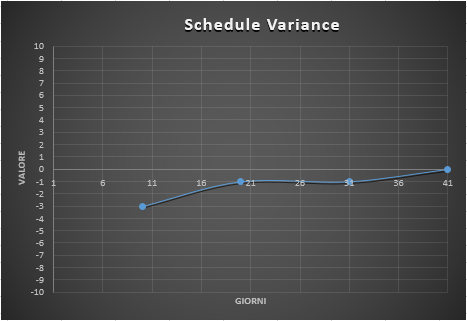
\includegraphics[scale=0.7]{Sezioni/Immagini/ScheduleVariance-RR}
	\caption{Schedule variance - RR}
\end{figure}

\begin{figure}[H]
	\centering 
	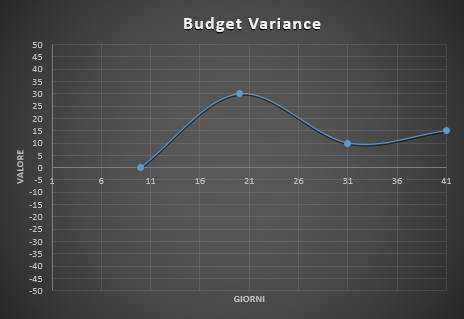
\includegraphics[scale=0.7]{Sezioni/Immagini/BudgetVariance-RR}
	\caption{Budget variance - RR}
\end{figure}

\subsubsection{Livello dei processi}
\begin{longtable}{|>{\centering}m{6cm}|c|c|c|c|c|}
\hline
\textbf{Processo} & \textbf{Livello} & \textbf{Esito} & \textbf{Valore}\\
\hline
\endhead
\emph{Processo di fornitura} & \textcolor{Green}{1} & Superato & Accettabile\\ \hline
\emph{Processo di sviluppo} & \textcolor{Green}{2}* & Superato & Accettabile\\ \hline
\emph{Processo di documentazione} & \textcolor{Green}{2} & Superato & Accettabile\\ 
\hline
\emph{Processo di Configurazione} & \textcolor{Green}{1} & Superato & Ottimale\\ 
\hline
\emph{Processo di garanzia di qualità del Prodotto} & * & / & /\\ 
\hline
\emph{Processo di Verifica} & \textcolor{Green}{1} & Superato & Ottimale\\ 
\hline
\emph{Processo di Validazione} & * & / & /\\ 
\hline
\emph{Processo di Risoluzione dei problemi} & \textcolor{Green}{1} & Superato & Ottimale\\ 
\hline
\emph{Processo di Coordinamento} & \textcolor{Green}{1} & Superato & Ottimale\\ 
\hline
\emph{Processo di Pianificazione} & \textcolor{Green}{1} & Superato & Ottimale\\ 
\hline
\emph{Processo di Formazione} & \textcolor{Green}{1} & Superato & Ottimale\\ 
\hline
\caption{RR-Livello dei processi}
\end{longtable}

Per i processi con segnatura \texttt{Voto*} vengono considerate solo le attività inerenti al lavoro che deve essere svolto per la \textit{Revisione di progettazione}. Per quelli, invece, con solo \texttt{*} significa che nessuna attività di quel processo era necessaria per il raggiungimento della milestone esterna.

\newpage

\subsection{Revisione di Progettazione}

\subsubsection{Analisi statica dei documenti}
L'analisi statica dei documenti è stata fatta mediante \termine{Walkthrough} ed ha portato all'individuazione di alcuni errori. Tra gli errori individuati quelli più frequenti sono stati:
		\begin{itemize}
			\item Errori ortografici.
			\item Parole con lettere mancanti o invertite.
			\item Periodi troppo lunghi o complessi da capire ed interpretare.
		\end{itemize}

\subsection{Metriche per i documenti}

\subsubsection{Indice di Gulpease}

\begin{table}[h]
	\begin{center}
		\begin{tabular}{|c|c|c|c|c|}
			\hline
			\textbf{Documento}	& \textbf{Risultato} & \textbf{Esito} & \textbf{Valore}\\
			\hline
		 \termine{Analisi} dei Requisiti v2.0.0 &	90 & Superato & Ottimale\\
			\hline
			Glossario v2.0.0 &	54 & Superato & Ottimale\\
			\hline
			Norme di Progetto v2.0.0 &	52 & Superato & Ottimale\\
			\hline
			Piano di Progetto v2.0.0	&	52 & Superato & Ottimale\\
			\hline
			Piano di Qualifica v2.0.0	&	46 & Superato & Accettabile\\
			\hline
			Definizione di \termine{Prodotto} v1.0.0	&	64 & Superato & Ottimale\\
			\hline
			Verbale\_Interno\_2\_20170222 v1.0.0	&	54 & Superato & Ottimale\\
			\hline
			Verbale\_Esterno\_3\_20170224 v1.0.0	&	53 & Superato & Ottimale\\
			\hline
			Verbale\_Interno\_4\_20170226 v1.0.0	&	51 & Superato & Ottimale\\
			\hline
			Verbale\_Interno\_5\_20170228 v1.0.0	&	52 & Superato & Ottimale\\
			\hline
		\end{tabular}
	\end{center}
	\caption{RP - Risultato indice di Gulpease}
\end{table}

\subsubsection{Soddisfacimento metriche}

\paragraph{Qualità di processo}
\begin{longtable}{|>{\centering}m{5cm}|c|c|c|c|c|}
\hline
\textbf{Metrica} & \textbf{Unità di misura} & \textbf{Risultato} & \textbf{Risultato Massimo} & \textbf{Esito} & \textbf{Valore}\\
\hline
\endhead

\emph{Schedule Variance} & {Attività} & \textcolor{Green}{0} & / & Superato & Ottimale\\ \hline
\emph{Budget Variance} & {Euro} & \textcolor{Orange}{-50} & / & Non superato & /\\ \hline
\emph{Ottimalità delle misurazioni} & {Percentuale} & \textcolor{Green}{0.6} & / & Superato & Ottimale \\ \hline
\emph{Rischi non preventivati} & {Rischi} & \textcolor{Green}{2} & / & Superato & Accettabile\\ \hline
%\emph{Efficienza di gestione dei rischi} & {Giorni} & \textcolor{Orange}{21.3} & $\geq 20$ & $\geq 60$\\ \hline
%\emph{Requisiti obbligatori soddisfatti} & {Percentuale} & \textcolor{Green}{100} & $100$ & $100$\\ \hline
\emph{Livello di instabilità-SDK} & {Percentuale} & / &\textcolor{Green}{1} & Superato & Accettabile\\ \hline
\emph{Livello di instabilità-Applicazione} & {Percentuale} & / &\textcolor{Green}{1} & Superato & Accettabile\\ \hline
\emph{Astrattezza-SDK} & {Percentuale} & \textcolor{Green}{0.8} & / & Superato & Accettabile\\ \hline
\emph{Astrattezza-Applicazione} & {Percentuale} & \textcolor{Green}{0.5} & / & Superato & Ottimale\\ \hline
\emph{Distanza dalla sequenza principale-SDK} & {Percentuale} & / &\textcolor{Green}{1} & Superato & Accettabile\\ \hline
\emph{Distanza dalla sequenza principale-Applicazione} & {Percentuale} & / &\textcolor{Green}{0.7} & Superato & Accettabile\\ \hline
\emph{Numero di metodi per classe} & {Metodi} & / &\textcolor{Green}{11} & Superato & Accettabile\\ \hline
\emph{Numero di attributi per classe} & {Attributi} & / &\textcolor{Green}{7} & Superato & Ottimale\\ \hline
\emph{Numero di parametri per metodo} & {Parametri} & / &\textcolor{Green}{7} & Superato & Ottimale\\ \hline
%\emph{Produttività di codifica} & {Linee} & \textcolor{Orange}{9.1} & $\geq 3$ & $\geq 10$\\ \hline
%\emph{Complessità Ciclomatica media} & {Cammini} & \textcolor{Green}{0} & $1 - 15$ & $1 - 10$\\ \hline
%\emph{Livelli di annidamento medi} & {Chiamate} & \textcolor{Green}{1} & $1 - 6$ & $1 - 3$\\ \hline
%\emph{Linee di codice per linee di commento} & {Percentuale} & \textcolor{Green}{31} & $\geq 25$ & $\geq 30$\\ \hline
%\emph{Variabili inutilizzate} & {Variabili} & \textcolor{Green}{0} & $0$ & $0$\\ \hline
%\emph{Dipendenze} & {Chiamate require} & \textcolor{Green}{2.2} & $0 - 10$ & $0 - 5$\\ \hline
%\emph{Halstead Difficulty media} & {Percentuale} & \textcolor{Green}{0} & $0 - 25$ & $0 - 15$\\ \hline
%\emph{Halstead Volume media} & {Percentuale} & \textcolor{Green}{20} & $20 - 1500$ & $20 - 1000$\\ \hline
%\emph{Halstead Effort media} & {Percentuale} & \textcolor{Green}{0} & $0 - 400$ & $0 - 300$\\ \hline
%\emph{Indice di manutenibilità} & {Percentuale} & \textcolor{Orange}{5.14} & $100 - 171$ & $120 - 171$\\ \hline
%\emph{Componenti integrate} & {Percentuale} & \textcolor{Green}{100} & $100$ & $100$\\ \hline
%\emph{Test di Unità eseguiti} & {Percentuale} & \textcolor{Red}{36.6} & $90 - 100$ & $100$\\ \hline
%\emph{Test di Integrazione eseguiti} & {Percentuale} & \textcolor{Red}{0} & $60 - 100$ & $70 - 100$\\ \hline
%\emph{Test di Sistema eseguiti} & {Percentuale} & \textcolor{Red}{0} & $70 - 100$ & $80 - 100$\\ \hline
%\emph{Test di \termine{Validazione} eseguiti} & {Percentuale} & \textcolor{Red}{0} & $100$ & $100$\\ \hline
%\emph{Test superati} & {Percentuale} & \textcolor{Green}{100} & $90 - 100$ & $100$\\ \hline
%\emph{Branch Coverage} & {Percentuale} & \textcolor{Orange}{73.3} & $70 - 100$ & $80 - 100$\\ \hline
%\emph{Code Coverage} & {Percentuale} & \textcolor{Green}{76.57} & $60 - 100$ & $70 - 100$\\ \hline
\caption{RP-Metriche di qualità di processo}
\end{longtable}

\subsubsection{Esiti delle metriche ripetute nel tempo}

\begin{figure}[H]
	\centering 
	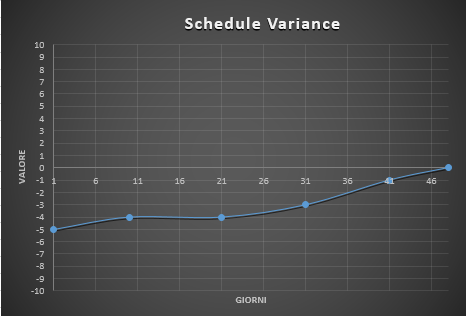
\includegraphics[scale=0.7]{Sezioni/Immagini/ScheduleVariance-RP}
	\caption{Schedule variance - RP}
\end{figure}

\begin{figure}[H]
	\centering 
	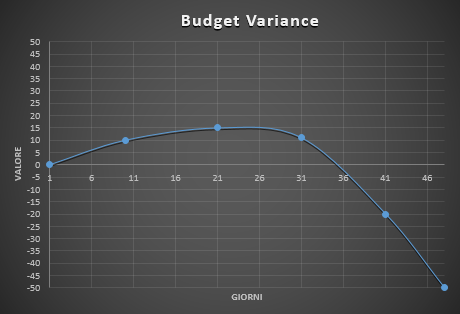
\includegraphics[scale=0.7]{Sezioni/Immagini/BudgetVariance-RP}
	\caption{Budget variance - RP}
\end{figure}

\begin{figure}[H]
	\centering 
	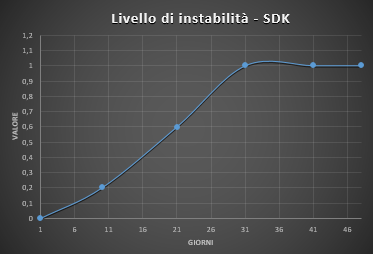
\includegraphics[scale=0.85]{Sezioni/Immagini/LivelloInstabilitaSDK-RP}
	\caption{Livello di instabilità SDK - RP}
\end{figure}

\begin{figure}[H]
	\centering 
	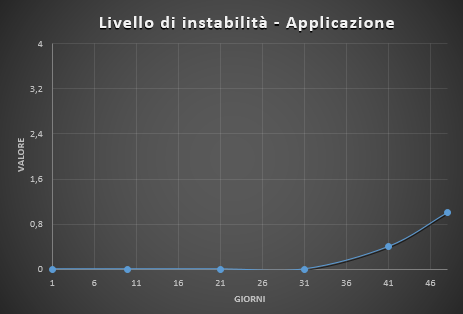
\includegraphics[scale=0.85]{Sezioni/Immagini/LivelloInstabilitaApp-RP}
	\caption{Livello di instabilità Applicazione - RP}
\end{figure}

\begin{figure}[H]
	\centering 
	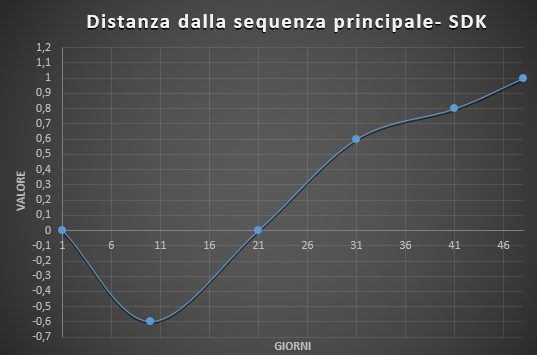
\includegraphics[scale=0.63]{Sezioni/Immagini/DistanzaSDK-RP}
	\caption{Distanza dalla sequenza principale SDK - RP}
\end{figure}

\begin{figure}[H]
	\centering 
	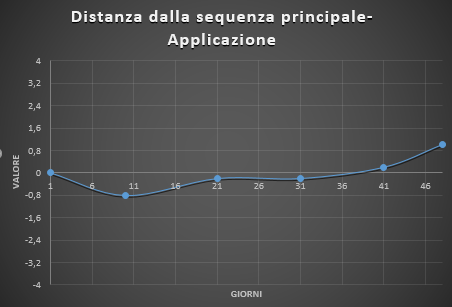
\includegraphics[scale=0.63]{Sezioni/Immagini/DistanzaApp-RP}
	\caption{Distanza dalla sequenza principale Applicazione - RP}
\end{figure}

\subsubsection{Livello dei processi}
\begin{longtable}{|>{\centering}m{6cm}|c|c|c|c|c|}
\hline
\textbf{Processo} & \textbf{Livello} & \textbf{Esito} & \textbf{Valore}\\
\hline
\endhead
\emph{Processo di fornitura} & \textcolor{Green}{2} & Superato & Ottimale\\ \hline
\emph{Processo di sviluppo} & \textcolor{Green}{2}* & Superato & Accettabile\\ \hline
\emph{Processo di documentazione} & \textcolor{Green}{2} & Superato & Accettabile\\ 
\hline
\emph{Processo di Configurazione} & \textcolor{Green}{1} & Superato & Ottimale\\ 
\hline
\emph{Processo di garanzia di qualità del Prodotto} & * & / & /\\ 
\hline
\emph{Processo di Verifica} & \textcolor{Green}{1} & Superato & Ottimale\\ 
\hline
\emph{Processo di Validazione} & * & / & /\\ 
\hline
\emph{Processo di Risoluzione dei problemi} & \textcolor{Green}{1} & Superato & Ottimale\\ 
\hline
\emph{Processo di Coordinamento} & \textcolor{Green}{1} & Superato & Ottimale\\ 
\hline
\emph{Processo di Pianificazione} & \textcolor{Green}{1} & Superato & Ottimale\\ 
\hline
\emph{Processo di Formazione} & \textcolor{Green}{1} & Superato & Ottimale\\ 
\hline
\caption{RP-Livello dei processi}
\end{longtable}

Per i processi con segnatura \texttt{Voto*} vengono considerate solo le attività inerenti al lavoro che deve essere svolto per la \textit{Revisione di progettazione}. Per quelli, invece, con solo \texttt{*} significa che nessuna attività di quel processo era necessaria per il raggiungimento della milestone esterna.

\newpage

\subsection{Revisione di Qualifica}

\subsubsection{Analisi statica dei documenti}
L'analisi statica dei documenti è stata fatta mediante \termine{Walkthrough} ed ha portato all'individuazione di alcuni errori. Tra gli errori individuati quelli più frequenti sono stati:
		\begin{itemize}
			\item Errori ortografici.
			\item Frasi complesse con un basso indice di comprensibilità.
		\end{itemize}

\subsection{Metriche per i documenti}

\subsubsection{Indice di Gulpease}

\begin{table}[h]
	\begin{center}
		\begin{tabular}{|c|c|c|c|c|}
			\hline
			\textbf{Documento}	& \textbf{Risultato} & \textbf{Esito} & \textbf{Valore}\\
			\hline
		    \termine{Analisi} dei Requisiti v3.0.0 & 87 & Superato & Ottimale\\
			\hline
			Glossario v3.0.0 & 55 & Superato & Ottimale\\
			\hline
			Norme di Progetto v3.0.0 & 46 & Superato & Accettabile\\
			\hline
			Piano di Progetto v3.0.0 & 48 & Superato & Accettabile\\
			\hline
			Piano di Qualifica v3.0.0 & 40 & Superato & Accettabile\\
			\hline
		 \termine{Manuale Utente} \termine{Monolith} v1.0.0 & 93 & Superato & Ottimale\\
			\hline
		 \termine{Manuale Utente} Bringit v1.0.0 & 48 & Superato & Accettabile\\
            \hline
            Verbale\_Interno\_7\_20170327 v1.0.0 & 67 & Superato & Ottimale\\
            \hline
            Verbale\_Interno\_8\_20170402 v1.0.0 & 73 & Superato & Ottimale\\
            \hline
            Verbale\_Interno\_9\_20170407 v1.0.0 & 78 & Superato & Ottimale\\
            \hline
            Verbale\_Esterno\_10\_20170503 v1.0.0 & 73 & Superato & Ottimale\\
            \hline
		\end{tabular}
	\end{center}
	\caption{RQ - Risultato indice di Gulpease}
\end{table}


\subsubsection{Soddisfacimento metriche}
\small{
Si noti che alcune componenti e i test a loro correlati non sono ancora state sviluppate, e che la loro assenza peserà nelle misurazioni.}

\paragraph{Qualità di processo}
\begin{longtable}{|>{\centering}m{5cm}|c|c|c|c|c|}
\hline
\textbf{Metrica} & \textbf{Unità di misura} & \textbf{Risultato} & \textbf{Risultato massimo} & \textbf{Esito} & \textbf{Valore}\\
\hline
\endhead
\emph{Schedule Variance} & {Attività} & \textcolor{Green}{0} & / & Superato & Ottimale\\ \hline
\emph{Budget Variance} & {Euro} & \textcolor{Orange}{-697} & / & Non superato & /\\ \hline
\emph{Ottimalità delle misurazioni} & {Percentuale} & \textcolor{Green}{74\%} & / & Superato & Ottimale \\ \hline
\emph{Rischi non preventivati} & {Rischi} & \textcolor{Green}{2} & / & Superato & Accettabile\\ \hline
\emph{Requisiti obbligatori soddisfatti} & {Percentuale} & \textcolor{Orange}{97.6\%} & / & Non superato & /\\ \hline
\emph{Livello di instabilità-SDK} & {Percentuale} & / & \textcolor{Green}{55\%} & Superato & Ottimale\\ \hline
\emph{Livello di instabilità-Applicazione} & {Percentuale} & / & \textcolor{Green}{70\%} & Superato & Accettabile\\ \hline
\emph{Astrattezza-SDK} & {Percentuale} & \textcolor{Green}{20\%} & / & Superato & Ottimale\\ \hline
\emph{Astrattezza-Applicazione} & {Percentuale} &\textcolor{Green}{15\%} & / & Superato & Ottimale\\ \hline
\emph{Distanza dalla sequenza principale-SDK} & {Percentuale} & / & \textcolor{Green}{25\%} & Superato & Ottimale\\ \hline
\emph{Distanza dalla sequenza principale-Applicazione} & {Percentuale} & / & \textcolor{Green}{15\%} & Superato & Ottimale\\ \hline
\emph{Numero di metodi per classe (max)} & {Metodi} & / & \textcolor{Green}{12} & Superato & Accettabile\\ \hline
\emph{Numero di attributi per classe (max)} & {Attributi} & / & \textcolor{Green}{7} & Superato & Ottimale\\ \hline
\emph{Numero di parametri per metodo (max)} & {Parametri} & / & \textcolor{Green}{5} & Superato & Ottimale\\ \hline
\emph{Complessità Ciclomatica media} & {Cammini} & \textcolor{Green}{1.3} & / & Superato & Ottimale\\ \hline
\emph{Livelli di annidamento medi} & {Chiamate} & \textcolor{Green}{2.4} & / & Superato & Ottimale\\ \hline
\emph{Linee di codice per linee di commento - Monolith} & {Percentuale} & \textcolor{Green}{28.3\%} & / & Superato & Ottimale\\ \hline
\emph{Linee di codice per linee di commento - BringIt} & {Percentuale} & \textcolor{Green}{20.5\%} & / & Superato & Ottimale\\ \hline
\emph{Componenti integrate} & {Percentuale} & \textcolor{Orange}{82\%} & / & Non superato & /\\ \hline
\emph{Test di Unità eseguiti} & {Percentuale} & \textcolor{Green}{99\%} & / & Superato & Ottimale\\ \hline
\emph{Test di Integrazione eseguiti} & {Percentuale} & \textcolor{Green}{84.7\%} & / & Superato & Ottimale\\ \hline
\emph{Test di Sistema eseguiti} & {Percentuale} & \textcolor{Green}{86\%} & / & Superato & Ottimale\\ \hline
\emph{Test di \termine{Validazione} eseguiti} & {Percentuale} & \textcolor{Orange}{46\%} & / & Non superato & / \\ \hline
\emph{Test superati} & {Percentuale} & \textcolor{Green}{100\%} & / & Superato & Ottimale \\ \hline
\emph{Branch Coverage} & {Percentuale} & \textcolor{Green}{83\%} & / & Superato & Accettabile\\ \hline
\emph{Statement Coverage} & {Percentuale} & \textcolor{Green}{77.4\%} & / & Superato & Accettabile\\ \hline
\emph{Accuratezza rispetto alle attese} & {Percentuale} & \textcolor{Green}{100} & / & Superato & Ottimale\\ \hline
\emph{Completezza dell’implementazione funzionale} & {Percentuale} & \textcolor{Orange}{86} & / & Non superato & /\\ \hline
\emph{Densità di failure} & {Percentuale} & \textcolor{Green}{0} & / & Superato & Ottimale\\ \hline
\emph{Blocco di operazioni non corrette} & {Percentuale} & \textcolor{Green}{90} & / & Superato & Accettabile\\ \hline
\emph{Tempo di risposta} & {Secondi} & / & \textcolor{Green}{1.0} & Superato & Ottimale\\ \hline
\emph{Capacità di analisi di failure} & {Percentuale} & \textcolor{Green}{100} & / & Superato & Ottimale\\ \hline
\emph{Impatto delle modifiche} & {Indice} & \textcolor{Green}{2} & / & Superato & Ottimale\\ \hline
\caption{RQ-Metriche di qualità di processo}\\
\end{longtable}

\subsubsection{Esiti delle metriche ripetute nel tempo}

\begin{figure}[H]
	\centering 
	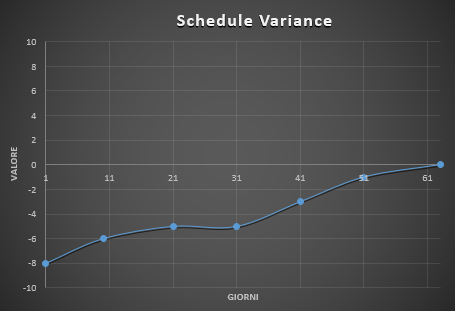
\includegraphics[scale=0.7]{Sezioni/Immagini/ScheduleVariance-RQ}
	\caption{Schedule variance - RQ}
\end{figure}

\begin{figure}[H]
	\centering 
	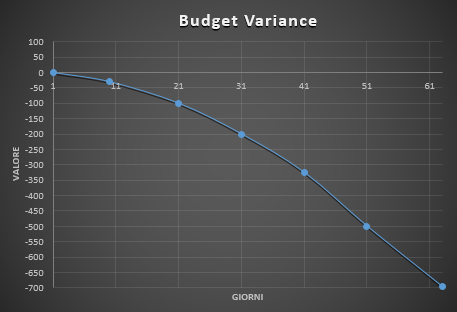
\includegraphics[scale=0.7]{Sezioni/Immagini/BudgetVariance-RQ}
	\caption{Budget variance - RQ}
\end{figure}

\begin{figure}[H]
	\centering 
	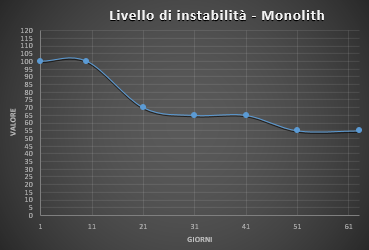
\includegraphics[scale=0.85]{Sezioni/Immagini/LivelloInstabilitaSDK-RQ}
	\caption{Livello di instabilità Monolith - RQ}
\end{figure}

\begin{figure}[H]
	\centering 
	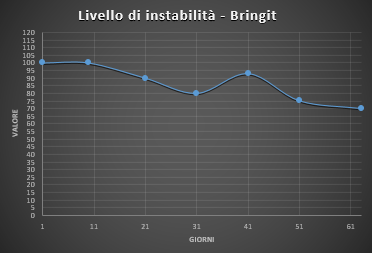
\includegraphics[scale=0.85]{Sezioni/Immagini/LivelloInstabilitaApp-RQ}
	\caption{Livello di instabilità Bringit - RQ}
\end{figure}

\begin{figure}[H]
	\centering 
	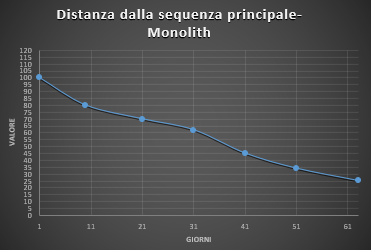
\includegraphics[scale=0.85]{Sezioni/Immagini/DistanzaSDK-RQ}
	\caption{Distanza dalla sequenza principale Monolith - RQ}
\end{figure}

\begin{figure}[H]
	\centering 
	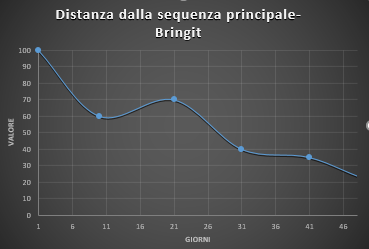
\includegraphics[scale=0.85]{Sezioni/Immagini/DistanzaApp-RQ}
	\caption{Distanza dalla sequenza principale Bringit - RQ}
\end{figure}

\begin{figure}[H]
	\centering 
	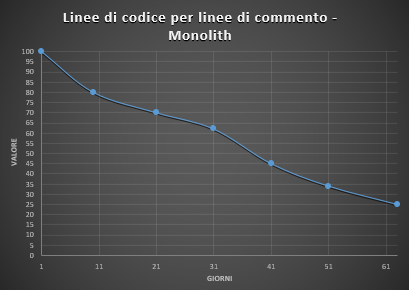
\includegraphics[scale=0.8]{Sezioni/Immagini/LineeCodiceCommentoSDK-RQ}
	\caption{Linee di codice per linee di commento Monolith - RQ}
\end{figure}

\begin{figure}[H]
	\centering 
	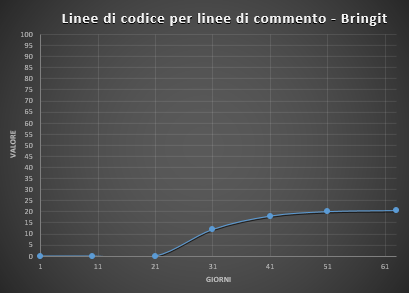
\includegraphics[scale=0.8]{Sezioni/Immagini/LineeCodiceCommentoApp-RQ}
	\caption{Linee di codice per linee di commento Bringit - RQ}
\end{figure}

\subsubsection{Livello dei processi}
\begin{longtable}{|>{\centering}m{6cm}|c|c|c|c|c|}
\hline
\textbf{Processo} & \textbf{Livello} & \textbf{Esito} & \textbf{Valore}\\
\hline
\endhead
\emph{Processo di fornitura} & \textcolor{Green}{2} & Superato & Ottimale\\ \hline
\emph{Processo di sviluppo} & \textcolor{Green}{2}* & Superato & Accettabile\\ \hline
\emph{Processo di documentazione} & \textcolor{Green}{2} & Superato & Accettabile\\ 
\hline
\emph{Processo di Configurazione} & \textcolor{Green}{1} & Superato & Ottimale\\ 
\hline
\emph{Processo di garanzia di qualità del Prodotto} & * & / & /\\ 
\hline
\emph{Processo di Verifica} & \textcolor{Green}{1} & Superato & Ottimale\\ 
\hline
\emph{Processo di Validazione} & * & / & /\\ 
\hline
\emph{Processo di Risoluzione dei problemi} & \textcolor{Green}{1} & Superato & Ottimale\\ 
\hline
\emph{Processo di Coordinamento} & \textcolor{Green}{1} & Superato & Ottimale\\ 
\hline
\emph{Processo di Pianificazione} & \textcolor{Green}{1} & Superato & Ottimale\\ 
\hline
\emph{Processo di Formazione} & \textcolor{Green}{1} & Superato & Ottimale\\ 
\hline
\caption{RQ-Livello dei processi}
\end{longtable}